\section{Experimental Methodology, Zero-Leakage Protocol, and Threats to Validity}
\label{sec:methodology_validity}

Empirical evaluations in automatic modulation classification (AMC) and adaptive edge computing are frequently undermined by subtle methodological flaws, including data snooping across overlapping frames, oracle leakage during feature extraction or attention conditioning, and uncalibrated latency claims \cite{sathyanarayanan2023rml22, wang2025survey}. To guarantee reproducible and scientifically sound findings, this section formalizes our unit of statistical independence, defines the zero-leakage information barrier, describes the hardware latency benchmark protocol, and details the threats to validity.

\subsection{Unit of Independence and Strict Partitioning}
\label{subsec:unit_independence}

In wireless signal classification, generating multiple observation windows by sliding or windowing a single continuous transmission creates severe autocorrelation in symbol sequences, fading state, carrier frequency offset (CFO), and noise realizations. When such windows are randomly split into training and test sets, deep neural networks exploit memorized channel signatures and symbol transitions rather than learning genuine modulation features---an artifact known as dataset contamination \cite{sathyanarayanan2023rml22}.

To eliminate this vulnerability, the fundamental and indivisible unit of statistical independence throughout our experimental framework is the \emph{parent waveform realization}, indexed by an immutable identifier $\texttt{parent\_waveform\_id} \in \mathcal{U}$. The end-to-end data generation process adheres to the following constraints:
\begin{enumerate}
    \item \textbf{Pre-Generation Partition Assignment:} The partition map $\mathcal{P}: \mathcal{U} \to \{\texttt{train}, \allowbreak \texttt{val\_cal}, \allowbreak \texttt{val\_policy}, \allowbreak \texttt{test}, \allowbreak \texttt{test\_shift}\}$ is determined prior to instantiating any physical signal parameters, symbol bits, channel coefficients, or noise vectors.
    \item \textbf{Hierarchical Deterministic PRNG Tree:} Randomness is governed hierarchically via \texttt{numpy.random.SeedSequence}. A master seed spawns isolated child seeds per partition, which subsequently derive unique seeds for each parent realization. This ensures that changing the seed or realization count in one partition preserves exact numerical bitstreams and realizations in all other partitions.
    \item \textbf{Strictly Disjoint Realizations:} 
    \begin{equation}
        \mathcal{U}_{\texttt{train}} \cap \mathcal{U}_{\texttt{val}} = \emptyset,\;
        \mathcal{U}_{\texttt{train}} \cap \mathcal{U}_{\texttt{test}} = \emptyset,\;
        \mathcal{U}_{\texttt{val}} \cap \mathcal{U}_{\texttt{test}} = \emptyset.
    \end{equation}
    No frames, sub-windows, or representations derived from the same parent waveform ever cross partition boundaries.
    \item \textbf{Exact Nested Prefix Alignment:} For every parent waveform realization $i \in \mathcal{U}$, the physical synthesizer produces a single continuous discrete-time sequence of $N_{\max} = 512$ samples $\mathbf{r}^{(i)}_{1:512}$. The short observation window $N_0 = 256$ is defined as the exact leading prefix:
    \begin{equation}
        \mathbf{r}^{(i)}_{1:256} = \mathbf{r}^{(i)}_{1:512}[0:256].
    \end{equation}
    Consequently, when an action switch occurs from $a_0$ to $a_1$, the classifier receives the exact temporal continuation of the channel, initial phase $\theta_0$, CFO $\Delta f$, and additive Gaussian noise realization $w[n]$, without artificial discontinuities or spliced independent realizations.
\end{enumerate}

The benchmark dataset comprises six balanced digital modulation schemes ($M \in \{\text{BPSK}, \text{QPSK}, \text{8PSK}, \text{16QAM}, \text{64QAM}, \text{4PAM}\}$) evaluated across eight nominal SNR operating points ($\text{SNR}_{\text{nom}} \in \{-20, -15, -10, -5, 0, +5, +10, +20\}\text{ dB}$) and varying RRC roll-off factors ($\beta \in \{0.25, 0.35, 0.50\}$). In-distribution (ID) partitions undergo random residual CFO $\Delta f \sim \mathcal{U}[-100, 100]\text{ Hz}$ and sparse discrete multipath channels with maximum excess delay up to 5 samples ($625\ \mu\text{s}$ at $f_s = 8\text{ kHz}$). The out-of-distribution (OOD) shift partition ($\texttt{test\_shift}$) evaluates extreme domain mismatch, incorporating severe CFO $|\Delta f| \in [200, 300]\text{ Hz}$ and extended sparse multipath profiles with excess delays of $9$ and $13$ samples (up to $1.625\text{ ms}$).

\subsection{Zero-Leakage Information Barrier}
\label{subsec:zero_leakage}

A pervasive defect in recent AMC literature involves the inadvertent leakage of oracle parameters to candidate models or decision routers. For instance, in MLEA-AMR \cite{gao2026mlea}, the true ground-truth SNR is supplied directly as a conditioning input to cross-attention layers; in Fewer-Sample \cite{guo2025fewer}, carrier frequency offset is artificially zeroed ($\Delta f = 0$), bypassing rotational synchronization; and in various deep learning frameworks, test-time batch statistics leak distributional information across samples via Batch Normalization.

Our framework enforces a strict \emph{zero-leakage information barrier} illustrated in Fig.~\ref{fig:information_barrier}:
\begin{figure}[!t]
\centering
\resizebox{\columnwidth}{!}{%
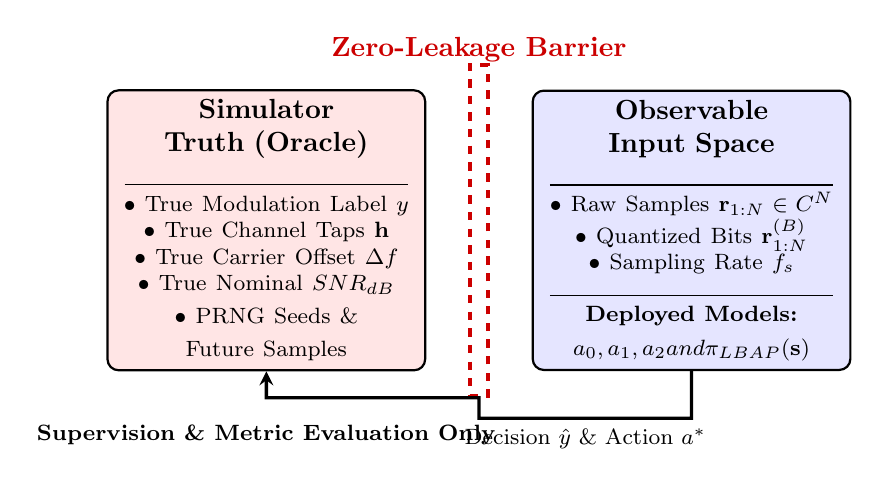
\begin{tikzpicture}[node distance=1.2cm, auto, >=stealth, thick]
    % Node definitions
    \node [draw, rectangle, fill=red!10, text width=3.8cm, text centered, rounded corners, minimum height=3.2cm] (oracle) {
        \textbf{Simulator Truth (Oracle)}\\
        \rule{3.6cm}{0.4pt}\\
        \footnotesize
        $\bullet$ True Modulation Label $y$\\
        $\bullet$ True Channel Taps $\mathbf{h}$\\
        $\bullet$ True Carrier Offset $\Delta f$\\
        $\bullet$ True Nominal $\text{SNR}_{\text{dB}}$\\
        $\bullet$ PRNG Seeds \& Future Samples
    };
    
    \node [draw, dashed, line width=1.5pt, red!80!black, minimum height=4.2cm, right of=oracle, node distance=2.7cm] (wall) {};
    \node [above of=wall, node distance=2.3cm, red!80!black] {\textbf{Zero-Leakage Barrier}};
    
    \node [draw, rectangle, fill=blue!10, text width=3.8cm, text centered, rounded corners, right of=wall, node distance=2.7cm, minimum height=3.2cm] (receiver) {
        \textbf{Observable Input Space}\\
        \rule{3.6cm}{0.4pt}\\
        \footnotesize
        $\bullet$ Raw Samples $\mathbf{r}_{1:N} \in \mathbb{C}^N$\\
        $\bullet$ Quantized Bits $\mathbf{r}^{(B)}_{1:N}$\\
        $\bullet$ Sampling Rate $f_s$\\
        \rule{3.6cm}{0.2pt}\\
        \textbf{Deployed Models:}\\
        $a_0, a_1, a_2 \text{ and } \pi_{\text{LBAP}}(\mathbf{s})$
    };
    
    % Flow arrows
    \draw [->, line width=1.2pt] (receiver.south) -- ++(0,-0.6) -| node[pos=0.25, below] {\footnotesize Decision $\hat{y}$ \& Action $a^*$} (wall.south) -| ++(-2.7,0) -- (oracle.south);
    \node at (0, -2.6) {\footnotesize \textbf{Supervision \& Metric Evaluation Only}};
\end{tikzpicture}%
}
\caption{Architectural representation of the zero-leakage information barrier. Candidate models ($a_0, a_1, a_2$) and the LBAP action selector operate strictly on observable complex baseband sequences $\mathbf{r}_{1:N}$ without access to oracle channel parameters, true CFO, nominal SNR, or future samples.}
\label{fig:information_barrier}
\end{figure}

\begin{enumerate}
    \item \textbf{Oracle Inaccessibility:} Neither the feature extraction pipelines (HOC, spectral moments), nor the deep neural networks ($a_2$), nor the action policy ($\pi_{\text{LBAP}}$) have access to true channel impulse responses $\mathbf{h}$, carrier offsets $\Delta f$, true SNR, symbol alignments, or future samples $n > N(a)$. All models consume exclusively the raw complex discrete-time observation vector $\mathbf{r}_{1:N} \in \mathbb{C}^N$ and the declared sampling rate $f_s$.
    \item \textbf{Blind Conditioning and SNR Independence:} When evaluating SNR-aware or spectral baselines (e.g., in policy input ablation), SNR is strictly replaced by a non-oracle, blind spectral estimate $\widehat{\text{SNR}}_{\text{blind}}$ derived from the ratio between total in-band power and the lower 35th percentile of periodogram power bins (exploiting the oversampling ratio $\text{sps} = 8$). True nominal SNR is strictly restricted to post-hoc stratification and visualization.
    \item \textbf{Causal Horizon and Temporal Non-Anticipation:} The decision to terminate acquisition at $N_0 = 256$ or proceed to $a_1$ ($N_1 = 512$) is computed strictly at physical time $t = 256 / f_s$ using features $\mathbf{s} \in \mathbb{R}^d$ computed solely from $\mathbf{r}_{1:256}$. The selector has zero lookahead into the future continuation $\mathbf{r}_{257:512}$.
    \item \textbf{Sample-Independent Inference (No Batch Normalization Leakage):} In multi-domain neural networks, standard Batch Normalization layers compute running minibatch statistics during evaluation if batch sizes exceed one, inadvertently allowing information to diffuse across distinct test examples. In $\text{MultiDomainAMCNet}$ ($a_2$), all normalization layers are strictly implemented via \texttt{GroupNorm} and \texttt{LayerNorm}. As formally verified in our regression test suite, single-sample evaluation ($\text{batch}=1$) produces mathematically identical activations and classification logits to batched execution, preserving sample-wise transductive isolation.
\end{enumerate}

\subsection{Latency Profiling and Virtual Acquisition Decomposition}
\label{subsec:latency_protocol}

Evaluating the computational overhead of adaptive edge architectures requires disentangling physical data collection from mathematical inference \cite{guo2025fewer, liu2026beacon}. In physical wireless receivers, the latency required to collect $N$ baseband samples across the antenna and analog-to-digital converter (ADC) interface is governed by the physical sampling rate:
\begin{equation}
    T_{\text{acq}}(a) = \frac{N(a)}{f_s}.
\end{equation}
The total execution delay for action $a \in \{a_0, a_1, a_2\}$ follows the sequential composition in Eq.~\eqref{eq:t_total_general} and \eqref{eq:t_comp_a0}--\eqref{eq:t_comp_a2}, namely $T_{\text{total}}(a) = T_{\text{acq}}(a) + T_{\text{comp}}(a)$, where routed computation includes the baseline prefix evaluation $T_{\text{base},0}$, gate latency $T_{\text{gate}}$, and any escalated model pass $T_{\text{base},a}$ ($a \in \{1,2\}$).

To prevent measurement distortion caused by operating system thread scheduling, dynamic CPU frequency throttling, and GPU kernel initialization, all latency benchmarks obey the following benchmarking protocol:
\begin{itemize}
    \item \textbf{Isolated Single-Sample Profiling:} Models are benchmarked in single-sample mode ($\text{batch}=1$) to replicate real-time streaming arrival at the edge.
    \item \textbf{Pre-Benchmark Warmup:} Classifiers execute eight complete warm-up forward passes on $\mathbf{r}_{1:N}$ prior to metric logging to warm up CPU L1/L2 caches, CUDA context structures, and memory allocators.
    \item \textbf{High-Resolution Timers:} Under single-thread contention controls (\texttt{threadpool\_limits(limits=1)}), profiling records isolated inference durations via nanosecond counters (\texttt{time.perf\_counter\_ns()}) across $96$ independent validation channel realizations repeated three times ($288$ recorded calls per model), reporting mean, median, and 95th-percentile (P95) latencies.
    \item \textbf{Sampling Rate Parametric Sweep:} Because physical RF bandwidth varies across IoT and radar standards (from narrowband sensor networks to wideband military radios), acquisition latency $T_{\text{acq}}$ is evaluated across four orders of magnitude: $f_s \in \{8\text{ kHz}, 32\text{ kHz}, 128\text{ kHz}, 1\text{ MHz}\}$.
\end{itemize}

\subsection{Threats to Validity}
\label{subsec:threats_validity}

To contextualize the scope of our conclusions and support transparent replication, we discuss the principal threats to validity affecting this investigation.

\subsubsection{Internal Validity}
Internal validity concerns the degree to which observed performance gains can be attributed causally to the proposed models rather than simulation artifacts.
\begin{itemize}
    \item \textbf{Discrete Baseband Channel Simplifications:} The signal propagation environment models linear multipath fading via discrete finite impulse response (FIR) tap-delay lines and carrier frequency offset via harmonic mixing. While this accurately captures frequency selectivity, intersymbol interference (ISI), and constellation spinning, it abstracts continuous-time Doppler spectra and non-linear analog RF front-end imperfections, including power amplifier (PA) saturation (AM/AM and AM/PM distortion), local oscillator (LO) phase noise, and I/Q mixer imbalances.
    \item \textbf{Static Frame Fading:} Multipath channel taps remain quasi-static over the duration of each 512-sample burst. Fast-fading channels where the coherence time is shorter than the observation window ($T_{\text{coh}} < 512 / f_s$) would induce time-varying dispersion that requires continuous adaptive equalization.
\end{itemize}

\subsubsection{Construct Validity}
Construct validity addresses whether our quantitative metrics accurately measure the theoretical constructs under study.
\begin{itemize}
    \item \textbf{Latency Proxies versus ASIC Hardware Implementations:} We measure algorithmic latency $T_{\text{calc}}$ on general-purpose commodity hardware (AMD/Intel multi-core CPUs and NVIDIA RTX GPUs). Although this reflects embedded software-defined radio (SDR) platforms, it serves as a proxy for dedicated Application-Specific Integrated Circuits (ASICs) or Field-Programmable Gate Arrays (FPGAs). As demonstrated by den Boer et al. \cite{denboer2021fpga}, pipelined FPGA neural accelerators achieve inference latencies of $3.71\ \mu\text{s}$ to $4.61\ \mu\text{s}$. In such microelectronic regimes, $T_{\text{calc}}$ becomes negligible compared to $T_{\text{acq}}$ at low-to-medium sampling rates ($f_s \le 128\text{ kHz}$), further amplifying the dominance of physical acquisition delay over arithmetic compute time.
    \item \textbf{Linear Utility Metric Formulation:} The net utility $U(a) = \mathbb{I}(\hat{y}=y) - \lambda T_{\text{total}}(a)$ employs a constant scalar penalty $\lambda$ to balance accuracy against delay. While mathematically tractable and standard in cost-sensitive learning \cite{liu2026beacon}, real-time mission-critical systems often feature non-linear, hard deadline constraints where utility drops to zero or negative infinity if processing exceeds an absolute time threshold $T_{\text{deadline}}$.
\end{itemize}

\subsubsection{External Validity}
External validity evaluates the generalizability of our findings to operational RF deployments.
\begin{itemize}
    \item \textbf{Modulation Alphabet Scope:} The experimental corpus investigates six fundamental single-carrier digital modulation schemes (BPSK, QPSK, 8PSK, 16QAM, 64QAM, 4PAM) commonly mandated in academic and military AMC benchmarks. Operational wireless ecosystems encounter multi-carrier waveforms (e.g., OFDM in 5G NR and IEEE 802.11), continuous phase modulations (CPFSK, MSK), and spread-spectrum signals (DSSS, FHSS).
    \item \textbf{ADC Quantization Architecture:} Our hardware-aware quantization study evaluates a uniform symmetric mid-rise ADC model across varying bit depths ($B \in \{8, 6, 5, 4\}$ bits) under fixed full-scale voltage ($V_{\text{FS}} = 2.5\text{ V}$). Although this provides direct insights into uniform dynamic range compression and SQNR degradation, it does not replicate the structural channel mismatches (gain mismatch, DC offset, and timing skew) characteristic of Time-Interleaved ADC (TI-ADC) topologies studied by Gros et al. \cite{gros2025mitigating}.
\end{itemize}
